\documentclass{standalone}
\usepackage{tikz}
\usetikzlibrary{patterns, positioning}


\begin{document}
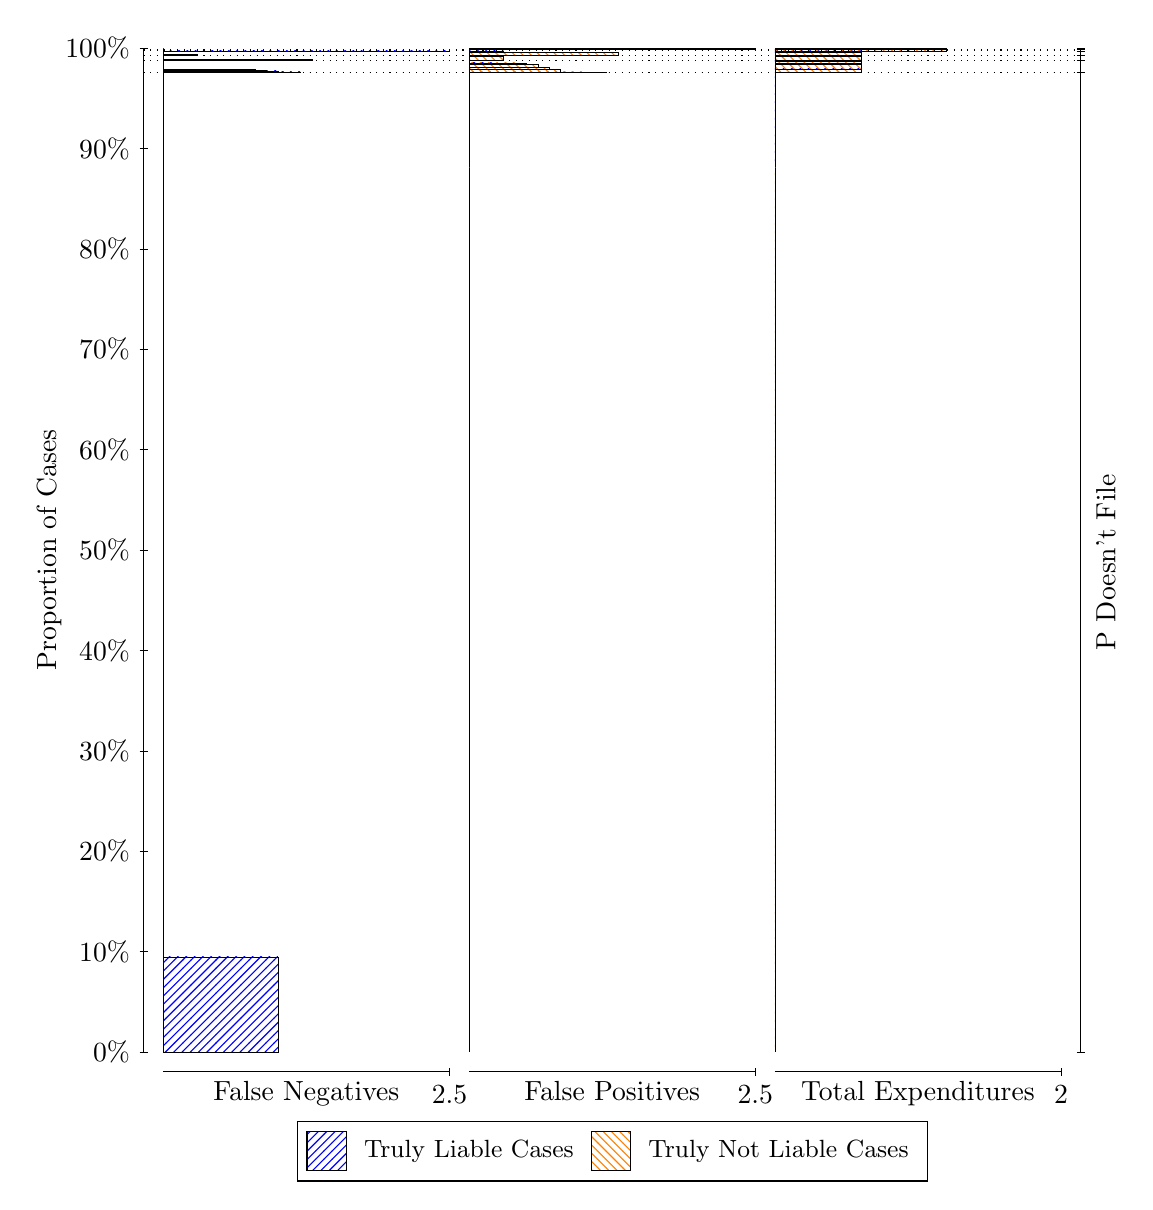
\begin{tikzpicture}
\draw[black, very thin] (1.5,1.75) -- (1.5,14.5);
\node[rotate=90, text=black, anchor=center] at (0.3, 8.125) {Proportion of Cases};
\draw[black, very thin] (1.45,1.75) -- (1.55,1.75);
\node[text=black, anchor=east] at (1.45, 1.75) {0\%};
\draw[black, very thin] (1.45,3.025) -- (1.55,3.025);
\node[text=black, anchor=east] at (1.45, 3.025) {10\%};
\draw[black, very thin] (1.45,4.3) -- (1.55,4.3);
\node[text=black, anchor=east] at (1.45, 4.3) {20\%};
\draw[black, very thin] (1.45,5.575) -- (1.55,5.575);
\node[text=black, anchor=east] at (1.45, 5.575) {30\%};
\draw[black, very thin] (1.45,6.85) -- (1.55,6.85);
\node[text=black, anchor=east] at (1.45, 6.85) {40\%};
\draw[black, very thin] (1.45,8.125) -- (1.55,8.125);
\node[text=black, anchor=east] at (1.45, 8.125) {50\%};
\draw[black, very thin] (1.45,9.4) -- (1.55,9.4);
\node[text=black, anchor=east] at (1.45, 9.4) {60\%};
\draw[black, very thin] (1.45,10.675) -- (1.55,10.675);
\node[text=black, anchor=east] at (1.45, 10.675) {70\%};
\draw[black, very thin] (1.45,11.95) -- (1.55,11.95);
\node[text=black, anchor=east] at (1.45, 11.95) {80\%};
\draw[black, very thin] (1.45,13.225) -- (1.55,13.225);
\node[text=black, anchor=east] at (1.45, 13.225) {90\%};
\draw[black, very thin] (1.45,14.5) -- (1.55,14.5);
\node[text=black, anchor=east] at (1.45, 14.5) {100\%};

\draw[black, very thin] (13.4,1.75) -- (13.4,14.5);
\draw[black, very thin] (13.35,1.75) -- (13.45,1.75);
\node[anchor=west] at (13.35, 1.75) {};
\draw[black, very thin] (13.35,14.191) -- (13.45,14.191);
\node[anchor=west] at (13.35, 14.191) {};
\draw[black, very thin] (13.35,14.194) -- (13.45,14.194);
\node[anchor=west] at (13.35, 14.194) {};
\draw[black, very thin] (13.35,14.344) -- (13.45,14.344);
\node[anchor=west] at (13.35, 14.344) {};
\draw[black, very thin] (13.35,14.405) -- (13.45,14.405);
\node[anchor=west] at (13.35, 14.405) {};
\draw[black, very thin] (13.35,14.463) -- (13.45,14.463);
\node[anchor=west] at (13.35, 14.463) {};
\draw[black, very thin] (13.35,14.486) -- (13.45,14.486);
\node[anchor=west] at (13.35, 14.486) {};
\draw[black, very thin] (13.35,14.5) -- (13.45,14.5);
\node[anchor=west] at (13.35, 14.5) {};

\draw[black, very thin, pattern color=blue, pattern=north east lines] (1.75,1.75) rectangle (3.2033,2.9571);
\draw[black, very thin, pattern color=orange, pattern=north west lines] (1.75,2.9571) rectangle (1.75,14.191);
\draw[black, very thin, pattern color=blue, pattern=north east lines] (1.75,14.191) rectangle (2.186,14.193);
\draw[black, very thin, pattern color=orange, pattern=north west lines] (1.75,14.193) rectangle (1.75,14.194);
\draw[black, very thin, pattern color=blue, pattern=north east lines] (1.75,14.194) rectangle (3.494,14.196);
\draw[black, very thin, pattern color=blue, pattern=north east lines] (1.75,14.196) rectangle (3.3487,14.198);
\draw[black, very thin, pattern color=blue, pattern=north east lines] (1.75,14.198) rectangle (3.2033,14.209);
\draw[black, very thin, pattern color=blue, pattern=north east lines] (1.75,14.209) rectangle (3.058,14.209);
\draw[black, very thin, pattern color=blue, pattern=north east lines] (1.75,14.209) rectangle (3.058,14.218);
\draw[black, very thin, pattern color=blue, pattern=north east lines] (1.75,14.218) rectangle (2.9127,14.227);
\draw[black, very thin, pattern color=blue, pattern=north east lines] (1.75,14.227) rectangle (2.7673,14.228);
\draw[black, very thin, pattern color=blue, pattern=north east lines] (1.75,14.228) rectangle (2.622,14.228);
\draw[black, very thin, pattern color=blue, pattern=north east lines] (1.75,14.228) rectangle (2.4767,14.228);
\draw[black, very thin, pattern color=blue, pattern=north east lines] (1.75,14.228) rectangle (2.3313,14.228);
\draw[black, very thin, pattern color=orange, pattern=north west lines] (1.75,14.228) rectangle (1.75,14.344);
\draw[black, very thin, pattern color=blue, pattern=north east lines] (1.75,14.344) rectangle (3.6393,14.355);
\draw[black, very thin, pattern color=orange, pattern=north west lines] (1.75,14.355) rectangle (1.75,14.405);
\draw[black, very thin, pattern color=blue, pattern=north east lines] (1.75,14.405) rectangle (2.186,14.421);
\draw[black, very thin, pattern color=orange, pattern=north west lines] (1.75,14.421) rectangle (1.75,14.463);
\draw[black, very thin, pattern color=blue, pattern=north east lines] (1.75,14.463) rectangle (5.3833,14.464);
\draw[black, very thin, pattern color=orange, pattern=north west lines] (1.75,14.464) rectangle (1.75,14.486);
\draw[black, very thin, pattern color=orange, pattern=north west lines] (1.75,14.486) rectangle (1.75,14.495);
\draw[black, very thin, pattern color=blue, pattern=north east lines] (1.75,14.495) rectangle (1.75,14.5);
\draw[black, very thin, pattern color=orange, pattern=north west lines] (5.6333,1.75) rectangle (5.6333,12.984);
\draw[black, very thin, pattern color=blue, pattern=north east lines] (5.6333,12.984) rectangle (5.6333,14.191);
\draw[black, very thin, pattern color=orange, pattern=north west lines] (5.6333,14.191) rectangle (7.0867,14.193);
\draw[black, very thin, pattern color=blue, pattern=north east lines] (5.6333,14.193) rectangle (5.6333,14.194);
\draw[black, very thin, pattern color=orange, pattern=north west lines] (5.6333,14.194) rectangle (7.3773,14.195);
\draw[black, very thin, pattern color=orange, pattern=north west lines] (5.6333,14.195) rectangle (7.232,14.195);
\draw[black, very thin, pattern color=orange, pattern=north west lines] (5.6333,14.195) rectangle (7.0867,14.197);
\draw[black, very thin, pattern color=orange, pattern=north west lines] (5.6333,14.197) rectangle (6.9413,14.198);
\draw[black, very thin, pattern color=orange, pattern=north west lines] (5.6333,14.198) rectangle (6.796,14.226);
\draw[black, very thin, pattern color=orange, pattern=north west lines] (5.6333,14.226) rectangle (6.6507,14.251);
\draw[black, very thin, pattern color=orange, pattern=north west lines] (5.6333,14.251) rectangle (6.5053,14.289);
\draw[black, very thin, pattern color=orange, pattern=north west lines] (5.6333,14.289) rectangle (6.36,14.303);
\draw[black, very thin, pattern color=orange, pattern=north west lines] (5.6333,14.303) rectangle (6.2147,14.31);
\draw[black, very thin, pattern color=blue, pattern=north east lines] (5.6333,14.31) rectangle (5.924,14.31);
\draw[black, very thin, pattern color=blue, pattern=north east lines] (5.6333,14.31) rectangle (5.7787,14.31);
\draw[black, very thin, pattern color=blue, pattern=north east lines] (5.6333,14.31) rectangle (5.6333,14.344);
\draw[black, very thin, pattern color=orange, pattern=north west lines] (5.6333,14.344) rectangle (6.0693,14.394);
\draw[black, very thin, pattern color=blue, pattern=north east lines] (5.6333,14.394) rectangle (5.6333,14.405);
\draw[black, very thin, pattern color=orange, pattern=north west lines] (5.6333,14.405) rectangle (7.5227,14.447);
\draw[black, very thin, pattern color=blue, pattern=north east lines] (5.6333,14.447) rectangle (6.0693,14.463);
\draw[black, very thin, pattern color=orange, pattern=north west lines] (5.6333,14.463) rectangle (5.6333,14.485);
\draw[black, very thin, pattern color=blue, pattern=north east lines] (5.6333,14.485) rectangle (5.6333,14.486);
\draw[black, very thin, pattern color=orange, pattern=north west lines] (5.6333,14.486) rectangle (9.2667,14.495);
\draw[black, very thin, pattern color=blue, pattern=north east lines] (5.6333,14.495) rectangle (7.8133,14.5);
\draw[black, very thin, pattern color=orange, pattern=north west lines] (9.5167,1.75) rectangle (9.5167,12.984);
\draw[black, very thin, pattern color=blue, pattern=north east lines] (9.5167,12.984) rectangle (9.5167,14.191);
\draw[black, very thin, pattern color=orange, pattern=north west lines] (9.5167,14.191) rectangle (10.062,14.193);
\draw[black, very thin, pattern color=blue, pattern=north east lines] (9.5167,14.193) rectangle (10.062,14.194);
\draw[black, very thin, pattern color=orange, pattern=north west lines] (9.5167,14.194) rectangle (10.607,14.224);
\draw[black, very thin, pattern color=blue, pattern=north east lines] (9.5167,14.224) rectangle (10.607,14.235);
\draw[black, very thin, pattern color=orange, pattern=north west lines] (9.5167,14.235) rectangle (10.607,14.295);
\draw[black, very thin, pattern color=blue, pattern=north east lines] (9.5167,14.295) rectangle (10.607,14.309);
\draw[black, very thin, pattern color=orange, pattern=north west lines] (9.5167,14.309) rectangle (10.607,14.335);
\draw[black, very thin, pattern color=blue, pattern=north east lines] (9.5167,14.335) rectangle (10.607,14.344);
\draw[black, very thin, pattern color=orange, pattern=north west lines] (9.5167,14.344) rectangle (10.607,14.394);
\draw[black, very thin, pattern color=blue, pattern=north east lines] (9.5167,14.394) rectangle (10.607,14.405);
\draw[black, very thin, pattern color=orange, pattern=north west lines] (9.5167,14.405) rectangle (10.607,14.447);
\draw[black, very thin, pattern color=blue, pattern=north east lines] (9.5167,14.447) rectangle (10.607,14.463);
\draw[black, very thin, pattern color=orange, pattern=north west lines] (9.5167,14.463) rectangle (11.697,14.485);
\draw[black, very thin, pattern color=blue, pattern=north east lines] (9.5167,14.485) rectangle (11.697,14.486);
\draw[black, very thin, pattern color=orange, pattern=north west lines] (9.5167,14.486) rectangle (11.697,14.495);
\draw[black, very thin, pattern color=blue, pattern=north east lines] (9.5167,14.495) rectangle (11.697,14.5);
\draw[black, dotted] (1.5,14.191) -- (13.4,14.191);
\draw[black, dotted] (1.5,14.194) -- (13.4,14.194);
\draw[black, dotted] (1.5,14.344) -- (13.4,14.344);
\draw[black, dotted] (1.5,14.405) -- (13.4,14.405);
\draw[black, dotted] (1.5,14.463) -- (13.4,14.463);
\draw[black, dotted] (1.5,14.486) -- (13.4,14.486);
\draw[black, very thin] (1.75,1.5) -- (5.3833,1.5);
\node[text=black, anchor=north] at (3.5667, 1.5) {False Negatives};
\draw[black, very thin] (5.3833,1.45) -- (5.3833,1.55);
\node[text=black, anchor=north] at (5.3833, 1.45) {2.5};

\draw[black, very thin] (5.6333,1.5) -- (9.2667,1.5);
\node[text=black, anchor=north] at (7.45, 1.5) {False Positives};
\draw[black, very thin] (9.2667,1.45) -- (9.2667,1.55);
\node[text=black, anchor=north] at (9.2667, 1.45) {2.5};

\draw[black, very thin] (9.5167,1.5) -- (13.15,1.5);
\node[text=black, anchor=north] at (11.333, 1.5) {Total Expenditures};
\draw[black, very thin] (13.15,1.45) -- (13.15,1.55);
\node[text=black, anchor=north] at (13.15, 1.45) {2};

\node[text=black, centered, rotate=90] at (13.72, 7.9707) {P Doesn't File};







\draw (7.449999999999999,1.5) node[draw=none] (baseCoordinate) {};
\begin{scope}[align=center]
        \matrix[scale=0.5, draw=black, below=0.5cm of baseCoordinate, nodes={draw}, column sep=0.1cm]{
            \node[rectangle, draw, minimum width=0.5cm, minimum height=0.5cm, pattern color=blue, pattern=north east lines] {}; &
            \node[draw=none, font=\small, text=black] (B) {Truly Liable Cases}; &
            \node[rectangle, draw, minimum width=0.5cm, minimum height=0.5cm, pattern color=orange, pattern=north west lines] {}; &
            \node[draw=none, font=\small, text=black] (B) {Truly Not Liable Cases}; \\
            };
\end{scope}

\end{tikzpicture}
\end{document}